Im ersten Schritt wird die Leerlaufspannung $U_\symup{0}$ einer Monozelle
gemessen. Hierfür werden die Anschlüsse des Voltmeters direkt mit den Anschlüssen
der Monozelle verbunden. Die angezeigte Spannung und der Innenwiderstand des
Voltmeters $R_\symup{i,V}$ werden notiert.
Nach dieser Messung werden ein Amperemeter und ein regelbarer Widerstand
$R_\symup{a}$, wie in Abbildung \ref{fig:schlt1}, mit der Monozelle in Reihe geschaltet.
\begin{figure}[H]
  \centering
  \begin{subfigure}{0.48\textwidth}
    \centering
    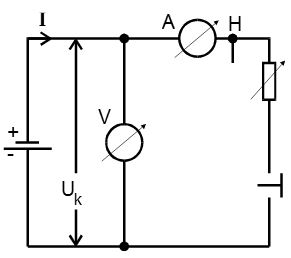
\includegraphics[width=4cm]{bilder/sinrecht.jpg}
    \caption{Messreihe 1}
    \label{fig:schlt1}
  \end{subfigure}
  \begin{subfigure}{0.48\textwidth}
    \centering
    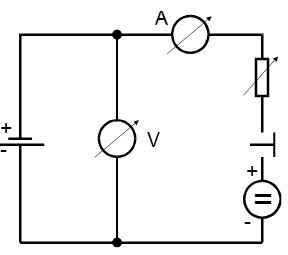
\includegraphics[width=4cm]{bilder/gegenspannung.jpg}
    \caption{Messreihe 2}
    \label{fig:schlt2}
  \end{subfigure}
  \caption{Schaltbilder \cite{301}}
  \label{fig:schlt}
\end{figure}
Das Voltmeter bleibt parallel geschaltet um den Spannungsverlauf über der
Monozelle zu messen. Der Widerstand wird hierbei von $(0-50)\Ohm$
variiert. Die Werte für $U_\symup{k}$ und $I$ werden notiert.
Abbildung \ref{fig:schlt2} zeigt die zweite Messreihe. Hier wird eine
Gegenspannung an die Monozelle gelegt. Die Gegenspannung ist $2\,\symup{\si{\volt}}$
größer als $U_\symup{0}$. Der Widerstand wird erneut von $(0-50)\,\symup{\si{\ohm}}$
variiert und die Werte für Strom und Spannung werden notiert.
Nach dieser Messung wird erneut die Schaltung aus \ref{fig:schlt1} aufgebaut.
Die Monozelle wird jedoch durch einen RC-Generator ersetzt. Dieser soll zunächst
eine Rechteckspannung liefern. Der Widerstand wird nun zwischen $(20-250)\,\symup{\si{\ohm}}$
variiert. Die Werte für $I$ und $U_\symup{k}$ werden an den Messgeräten
abgelesen und notiert.
Die Messung wird mit einer Sinusspannung und einem Widerstand von
$(0,1-5)\,\symup{\si{\kilo\ohm}}$ wiederholt.
\newpage
